\section{Pre-trained Encoders with a Simple Decoder}
In this first part of the project the pre-trained encoders of the \verb|VGG16|, the \verb|MobileNetV2| and the \verb|ResNet50V2| were chosen out of the available models in the keras software (\url{https://keras.io/api/applications}). These CNNs were selected due to their broad use in other open projects and their further development. Furthermore, the encoder of the three CNN differ a lot in the amount of weights (see \cref{tab:ParameterSummary} and it could thereby be evaluated if deeper encoder and therefore deeper CNN perform better in this task. In order to compare these different encoders, a simple decoder (code found in \cref{lst:simpleDecoder}) as shown in \cref{fig:architetcture_simple_decoder} was applied to each of the encoders in order to yield a CNN for the first tests in this project.\\
\begin{minipage}[t]{\textwidth}
\centering
	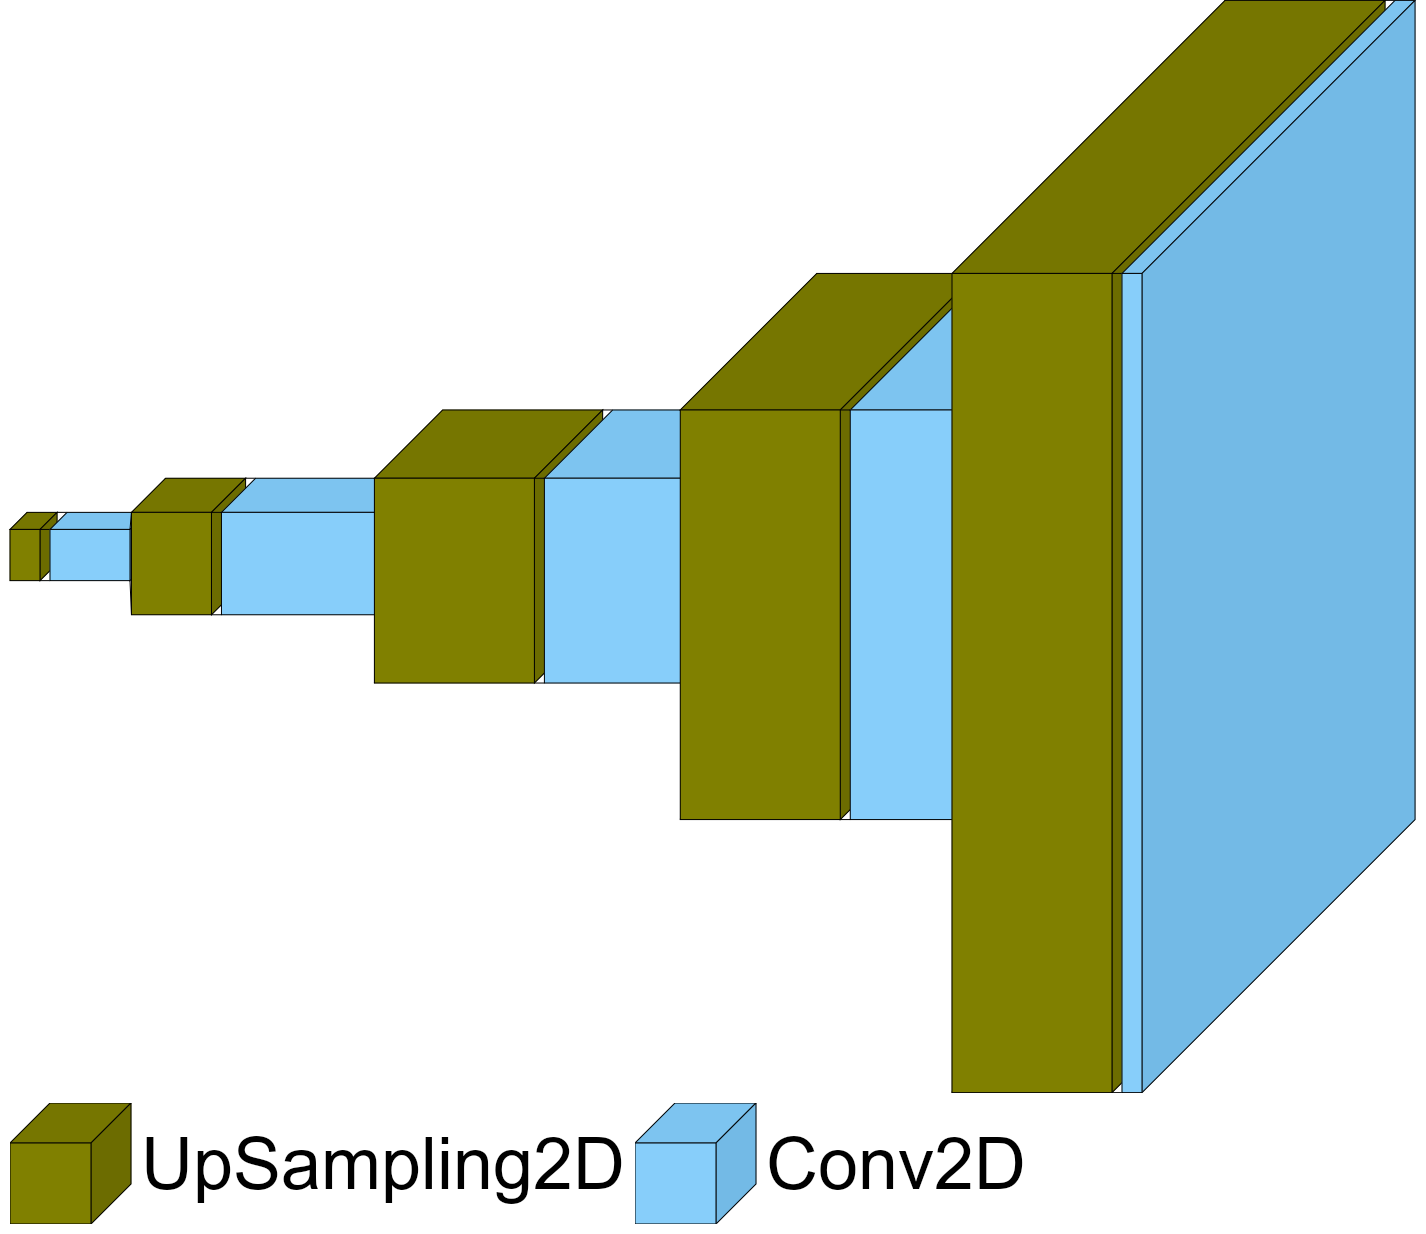
\includegraphics[width=0.5\textwidth]{Images/model_plot/simple_decoder.png}
	\captionof{figure}{Architecture of simple decoder}
	\label{fig:architetcture_simple_decoder}
\end{minipage}

\subsection{VGG16}
This CNN was build for the ImageNet Challenge 2014 for image classification and localisation \cite{simonyan2015deep}. This is why it is the the oldest architecture. The objective was to develop deeper CNN architectures, here with 23 weigh layer and over 14.700.000 parameters. Its size lays between the \verb|ResNet50V2| and the \verb|MobileNetV2| regarding the amount of parameters.\\

\begin{minipage}[t]{\textwidth}
    %\vspace{5mm}
    \centering
	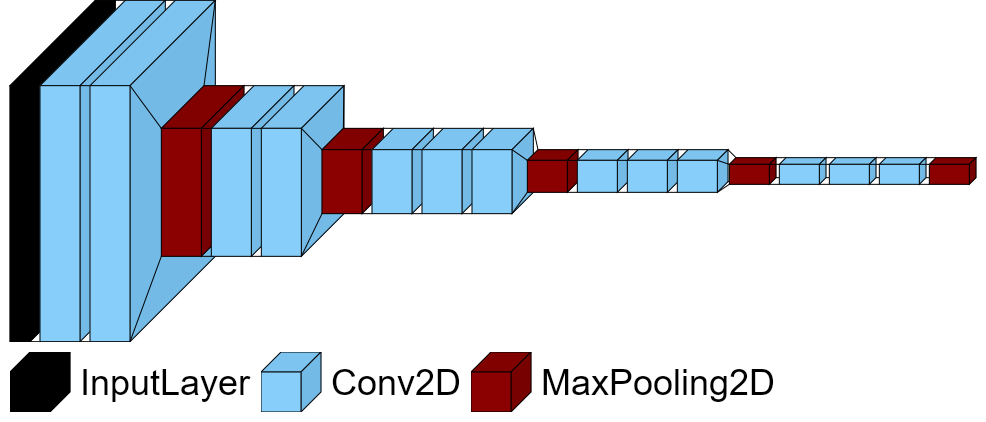
\includegraphics[width=0.7\textwidth]{Images/model_plot/vgg16.png}
	\captionof{figure}{Architecture of VGG16}
	\label{fig:architetcture_vgg16}
	\vspace{5mm}
\end{minipage}
	
\subsection{MobileNetV2}
The \verb|MobileNetV2|, introduced in \cite{sandler2019mobilenetv2}, was build and improved in order to obtain a small mobile model for semantic segmentation. It is the smallest pre-trained model and also the latest model used in this project. It contains around 2.400.000 parameters in 88 layers.\\

\begin{minipage}[t]{\textwidth}
	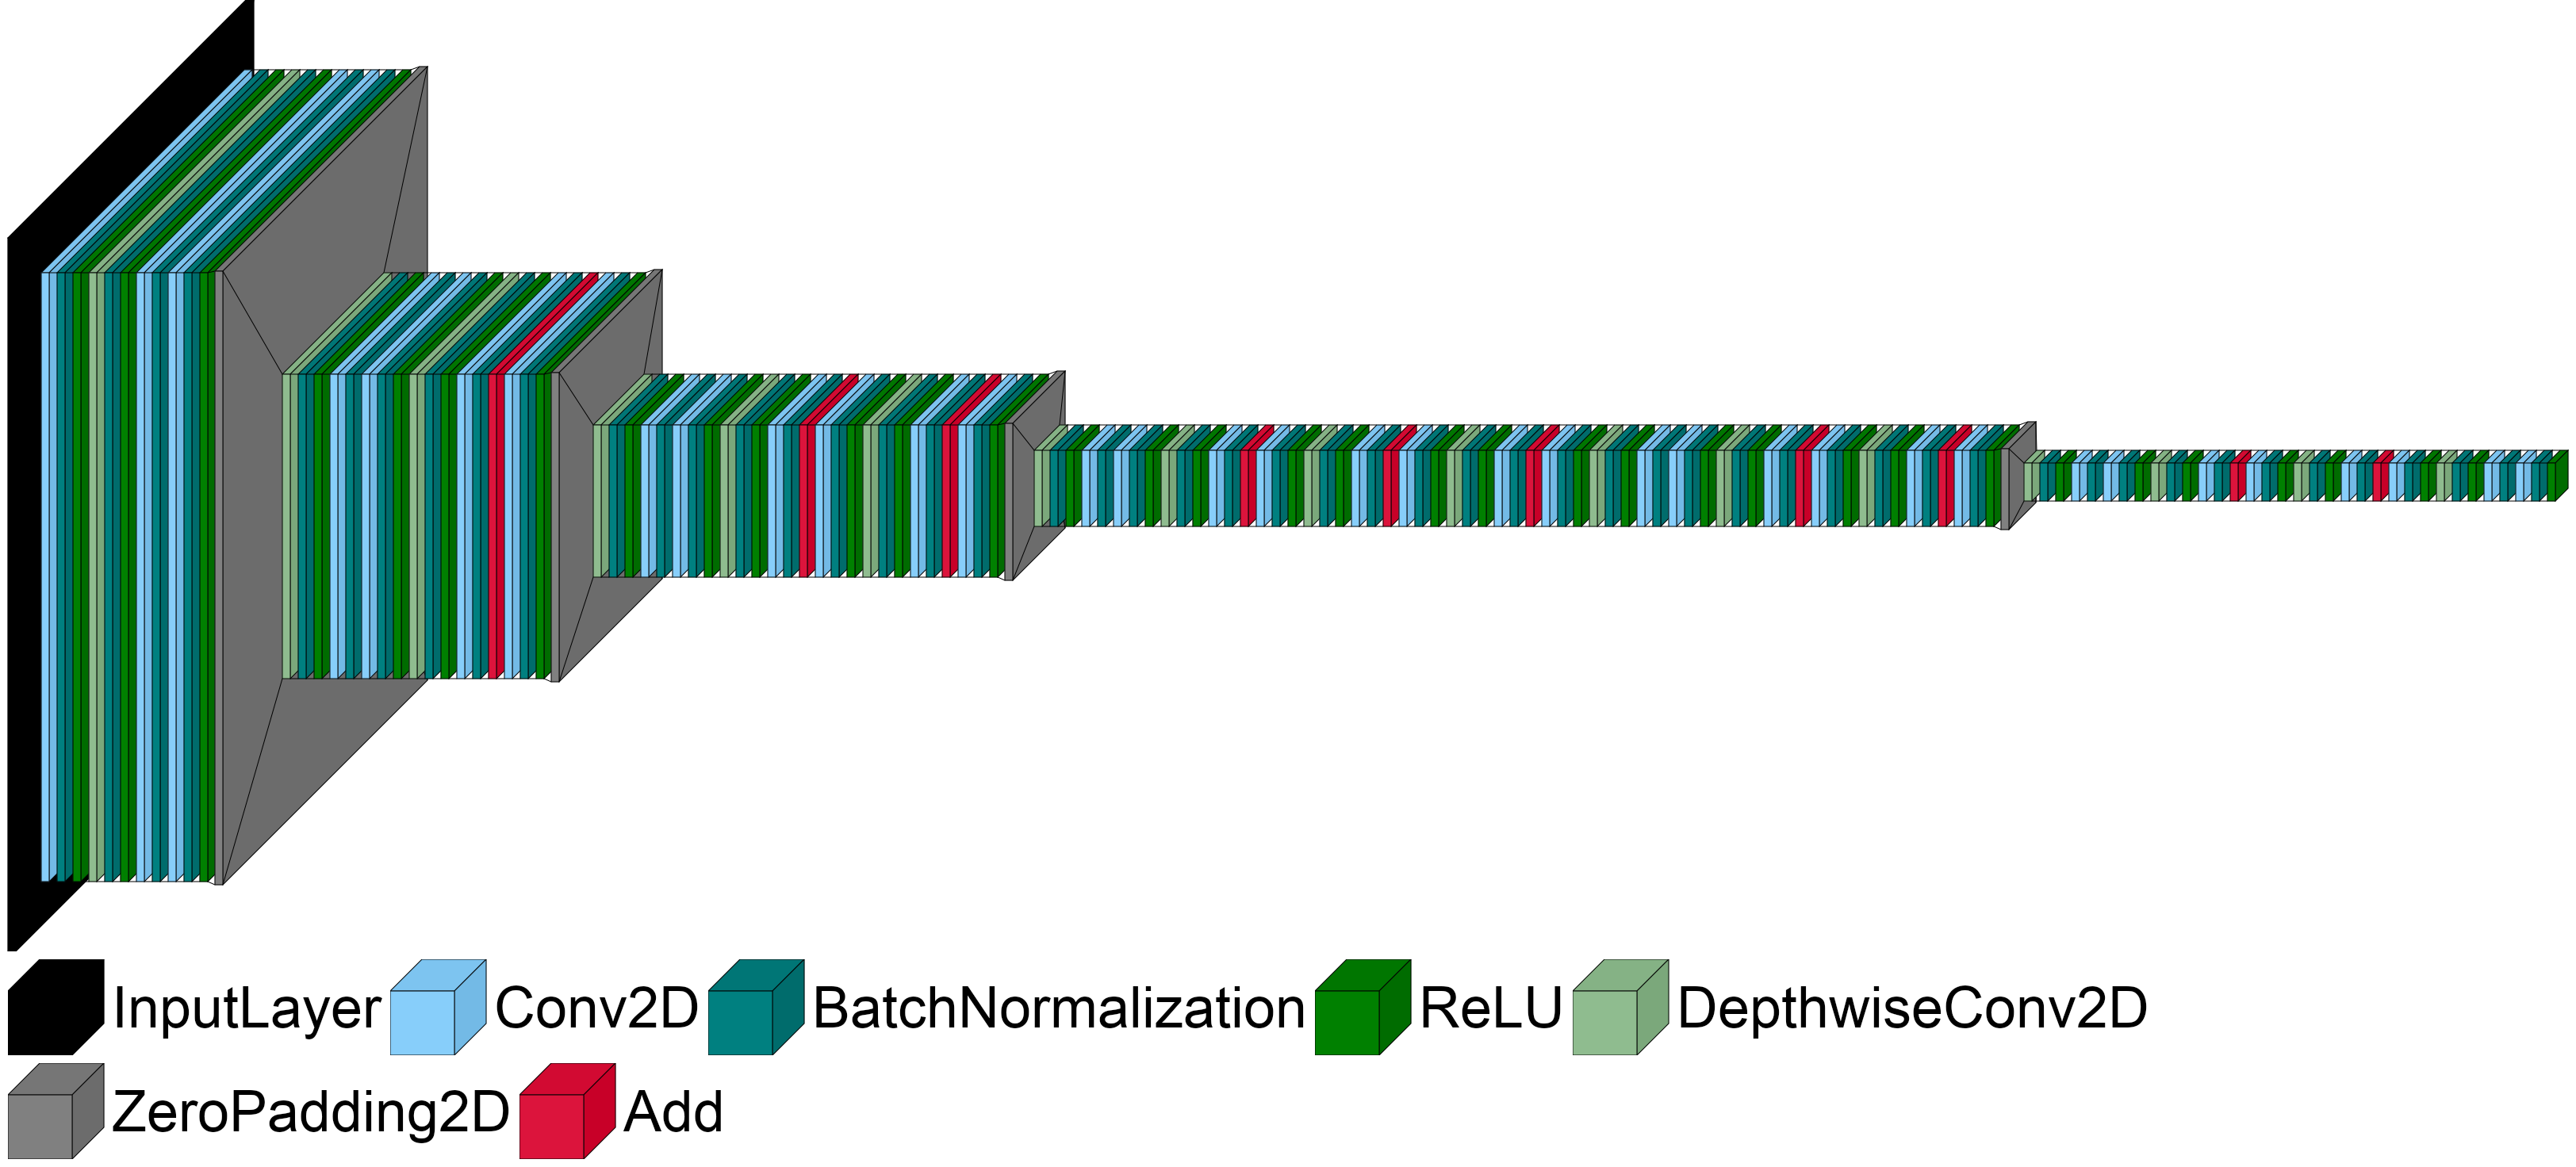
\includegraphics[width=\textwidth]{Images/model_plot/mobilenet_v2.png}
	\captionof{figure}{Architecture of MobileNetV2}
	\label{fig:architetcture_mobilenet_v2}
\end{minipage}

\subsection{ResNet50V2}
The \verb|ResNet50V2| architecture was build in order to ease the training of deep CNN (see \cite{He_2016_CVPR}) by using layers as residual functions regarding the input. The \verb|ResNet50V2| is the biggest segmentation net encoder used in this project regarding the amount of parameters. It contains around 23.700.000 parameters.\\

\begin{minipage}[t]{\textwidth}
	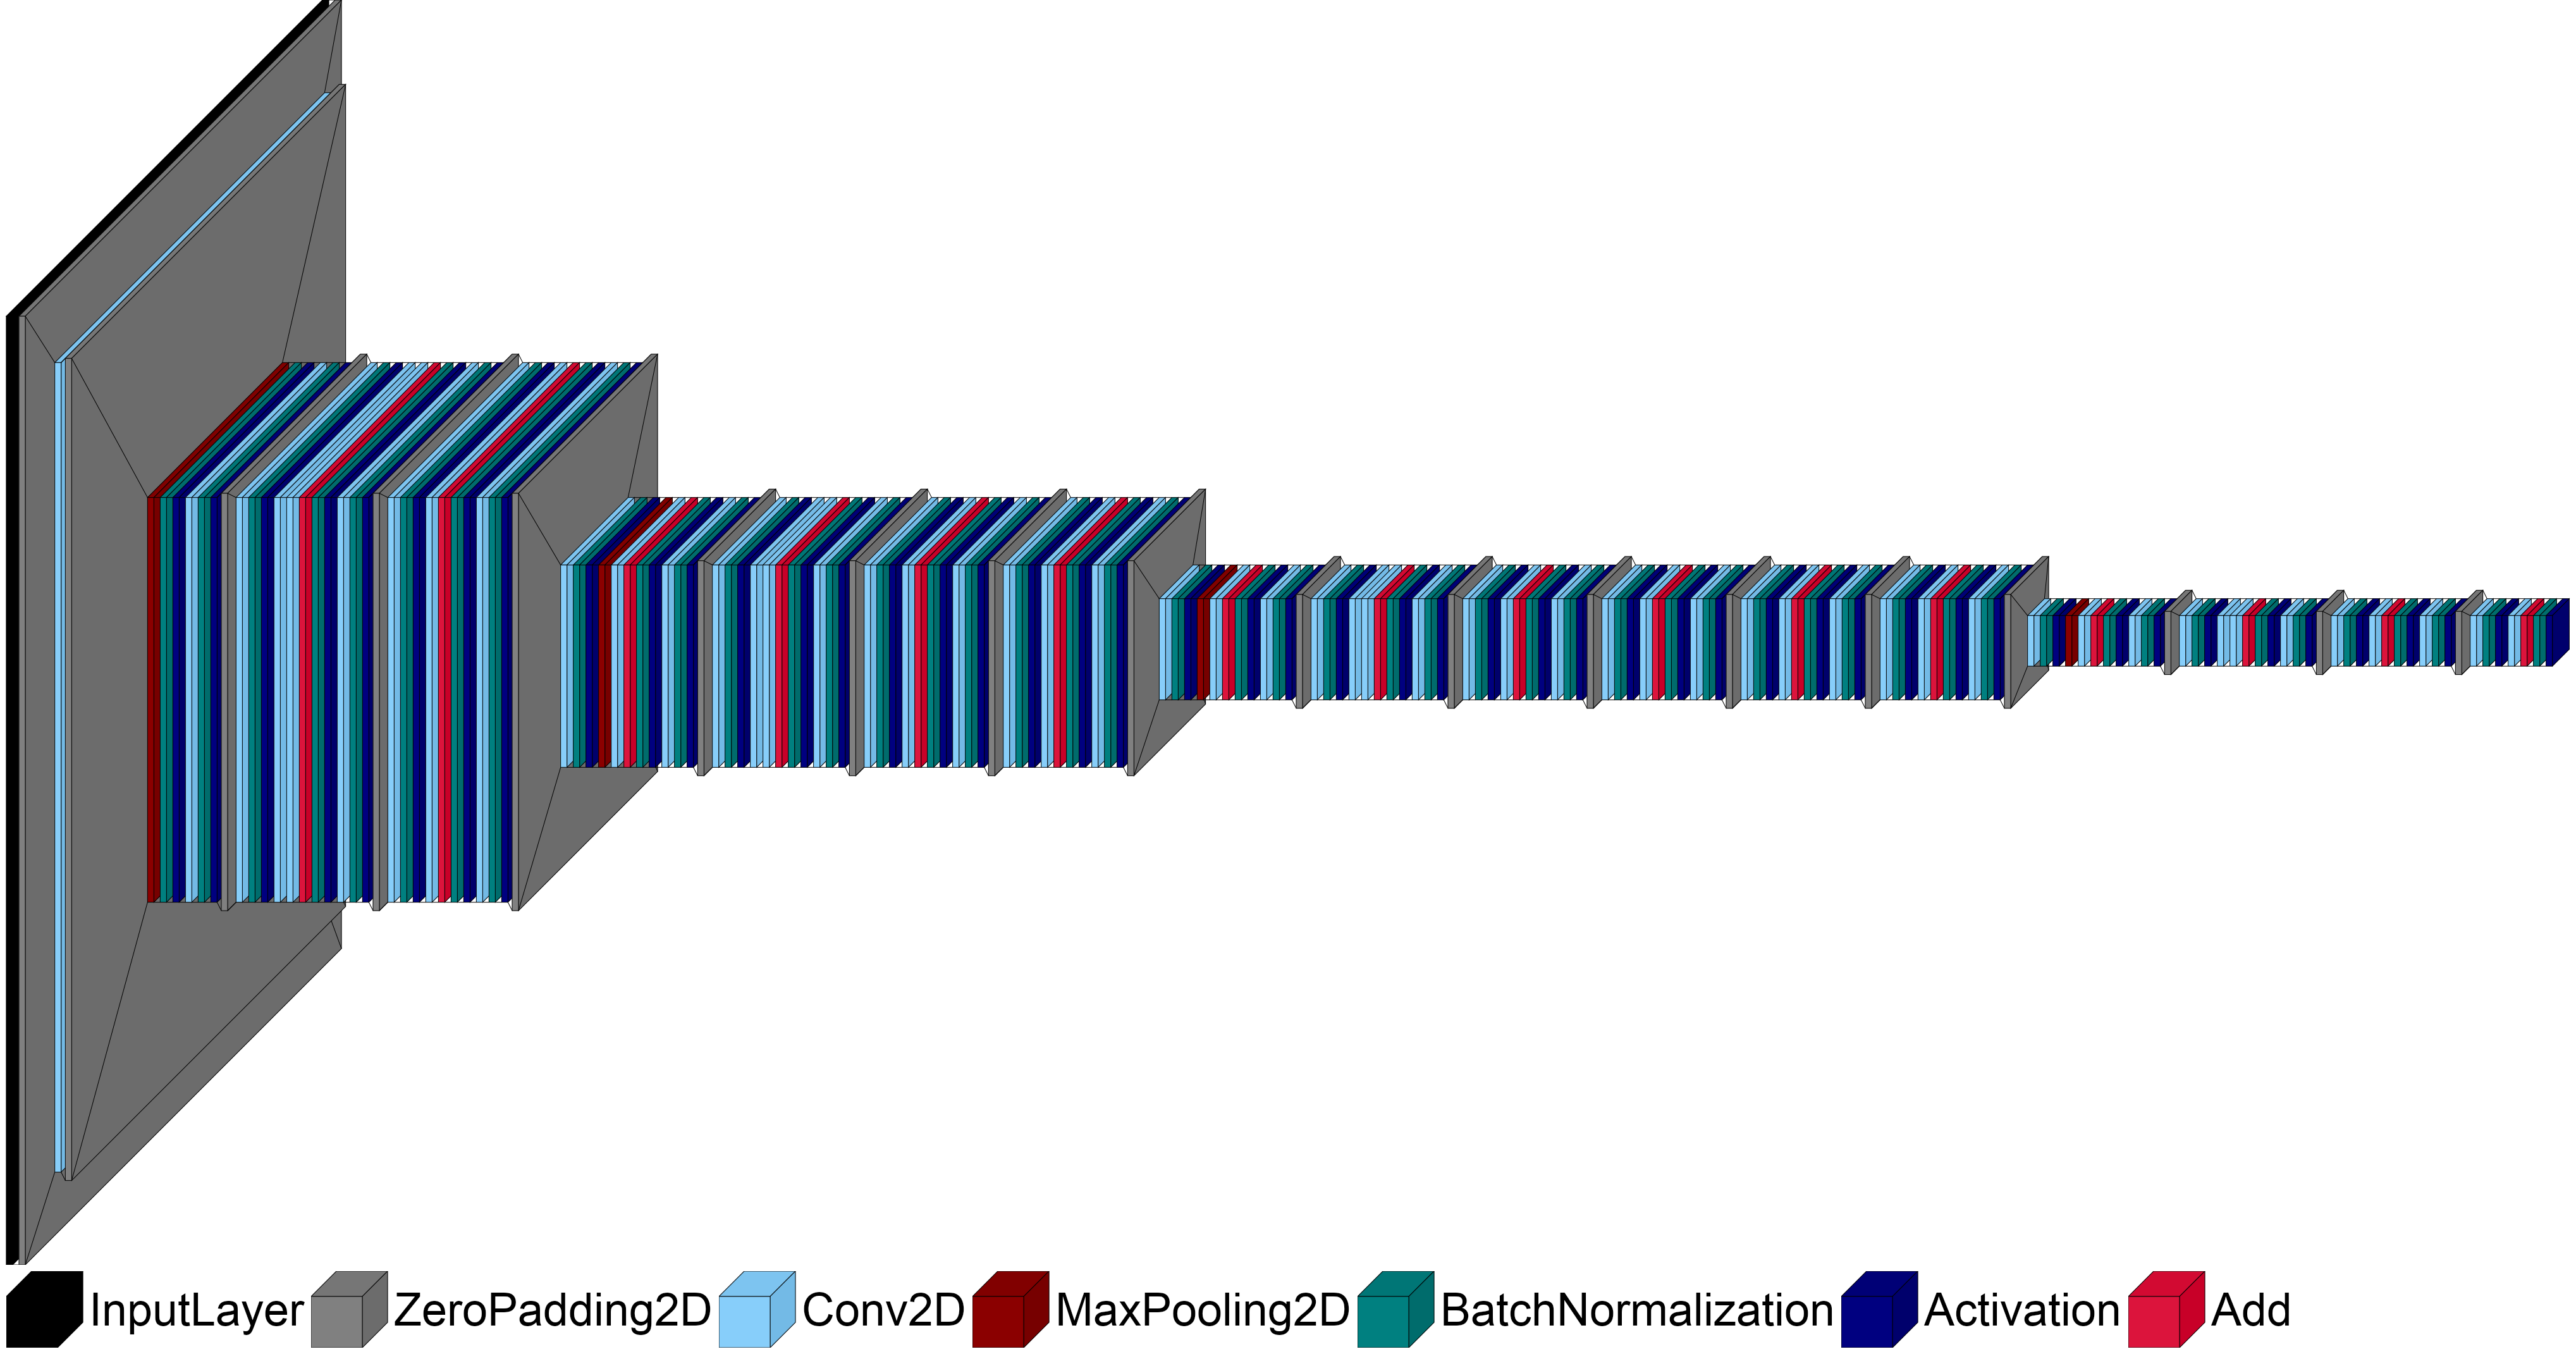
\includegraphics[width=\textwidth]{Images/model_plot/resnet.png}
	\captionof{figure}{Architecture of ResNet50V2}
	\label{fig:architetcture_resnet}
\end{minipage}

\section{Advanced Net Architectures and Decoder}
In this second part of the project, different architectures of segmentation nets are tested. Because of the different difficulties in every architecture, not all CNN performed the same test cases. So, several different settings in each investigation are applied.

\subsection{SegNet Architecture}
The SegNet Architecture in \cite{Badrinarayanan.2017} was created for a good segmentation performance while using fewer parameters. This is achieved by using max-pooling indices from the encoder for the up-sampling in the decoder. It was motivated for scene understanding applications.\\
In order to accelerate the training of the SegNet, a reduced architecture with fewer parameters than in the setup of \cite{Badrinarayanan.2017} is considered (see \cref{fig:architetcture_segnet}). The SegNet architecture can be extended by adding more blocks of \verb|Conv2D|, \verb|BatchNormalization| and \verb|Activation| before the \verb|MaxPoolingWithIndices| is performed. The presented implementation below is based on existing setups using keras (see \url{https://github.com/danielenricocahall/Keras-SegNet} and \url{https://github.com/Runist/SegNet-keras}).\\

\begin{minipage}[t]{\textwidth}
    %\vspace{5mm}
    \centering
    \hspace{-1cm}
	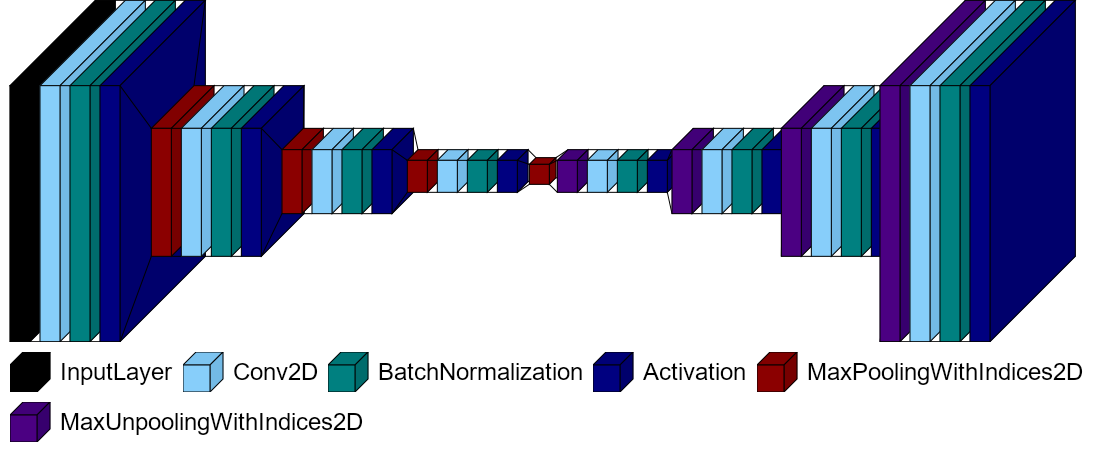
\includegraphics[width=\textwidth]{Images/model_plot/segnet.png}
	\captionof{figure}{Architecture of simplified SegNet}
	\label{fig:architetcture_segnet}
	\vspace{5mm}
\end{minipage}\\
In contrast to the other models that are presented within the scope of this project, the SegNet requires the use of layers that are not predefined in \verb|Keras| for the use of the mentioned max-pooling indices. This concerns \verb|MaxPoolingWithIndices2D| and \verb|MaxUnppolingWithIndices2D|.

\subsection{U-Net Architecture}
The U-Net architecture was motivated by biological image segmentation and the winning segmentation net in the ISBI challenge 2015. Similar to the SegNet, it applies encoder feature maps to the decoder in order to use trained feature maps more efficiently. With this approach, the U-Net presented in \cite{Ronneberger.2015} could achieve very good results by using only little data for the training.\\

\begin{minipage}[t]{\textwidth}
	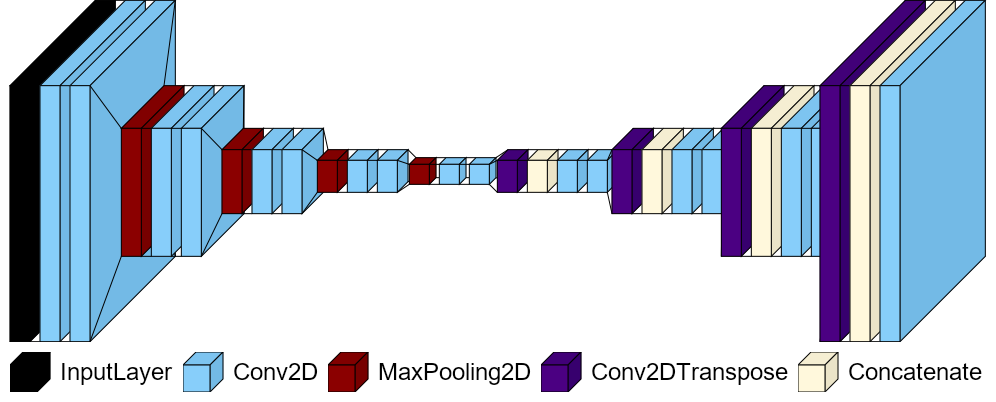
\includegraphics[width=\textwidth]{Images/model_plot/unet.png}
	\captionof{figure}{Architecture of U-Net with complexity of 4}
	\label{fig:architetcture_unet}
\end{minipage}

\subsection{Advanced Decoders}
Starting with the simple decoder in the first part of the project (\cref{lst:simpleDecoder}), more complex decoders were created and tested. In order to have more parameters for the learning, additional layers like \verb|Upsampling|, \verb|Conv2D|, \verb|Conv2DTranspose|, \verb|BatchNormalization|, \verb|Activation|, \verb|Add| and \verb|Dropout| are applied in the decoder architecture. Different combinations are tested as well as an architecture inspired by the examples for Computer Vision (\url{https://keras.io/examples/vision/oxford_pets_image_segmentation/}). The encoder used for these investigations is the \verb|MobileNetV2|, because of its fewer parameters and therefore faster training and prediction. The most important test are shown in this report:\\

    \begin{itemize}
    \item Multi- \& Single-Class Segm. with \verb|MobileNetV2| using
    \verb|Conv2DTranspose| with and without \verb|BatchNormalization|
    \item Multi- \& Single-Class with \verb|MobileNetV2| using
    two \verb|Conv2D| while \verb|Add| an \verb|Upsampling|, seen in \cref{lst:Decoder-Upsampling}
    \item Multi- \& Single-Class with \verb|MobileNetV2| using
    \verb|Conv2DTranspose| while \verb|Add| an \verb|Upsampling|, seen in \cref{lst:Decoder-Transpose}
    \item Multi- \& Single-Class with \verb|MobileNetV2| using
    \verb|Dropout| while \verb|Add| an \verb|Upsampling|, seen in \cref{lst:Decoder-Dropout}
    \item Multi- \& Single-Class with \verb|MobileNetV2| using
    two paths with different layer structures, seen in \cref{lst:Decoder-AdvancedDecoder}.
    \end{itemize}
\vspace{1cm}
n \cref{lst:Decoder-AdvancedDecoder} the decoder structure for the most advanced case is shown. In all of these tests of advanced decoders, five layers were applied in the decoder. These layers were built always exactly the same and similarly but simpler to the here shown structure. They all consisted  of an addition of an \verb|Upsampling| and another path including more parameters. Before the paths were added a \verb|BatchNormalization| and an \verb|Activation| were computed.\\

\begin{minipage}[t]{\textwidth}
\centering
	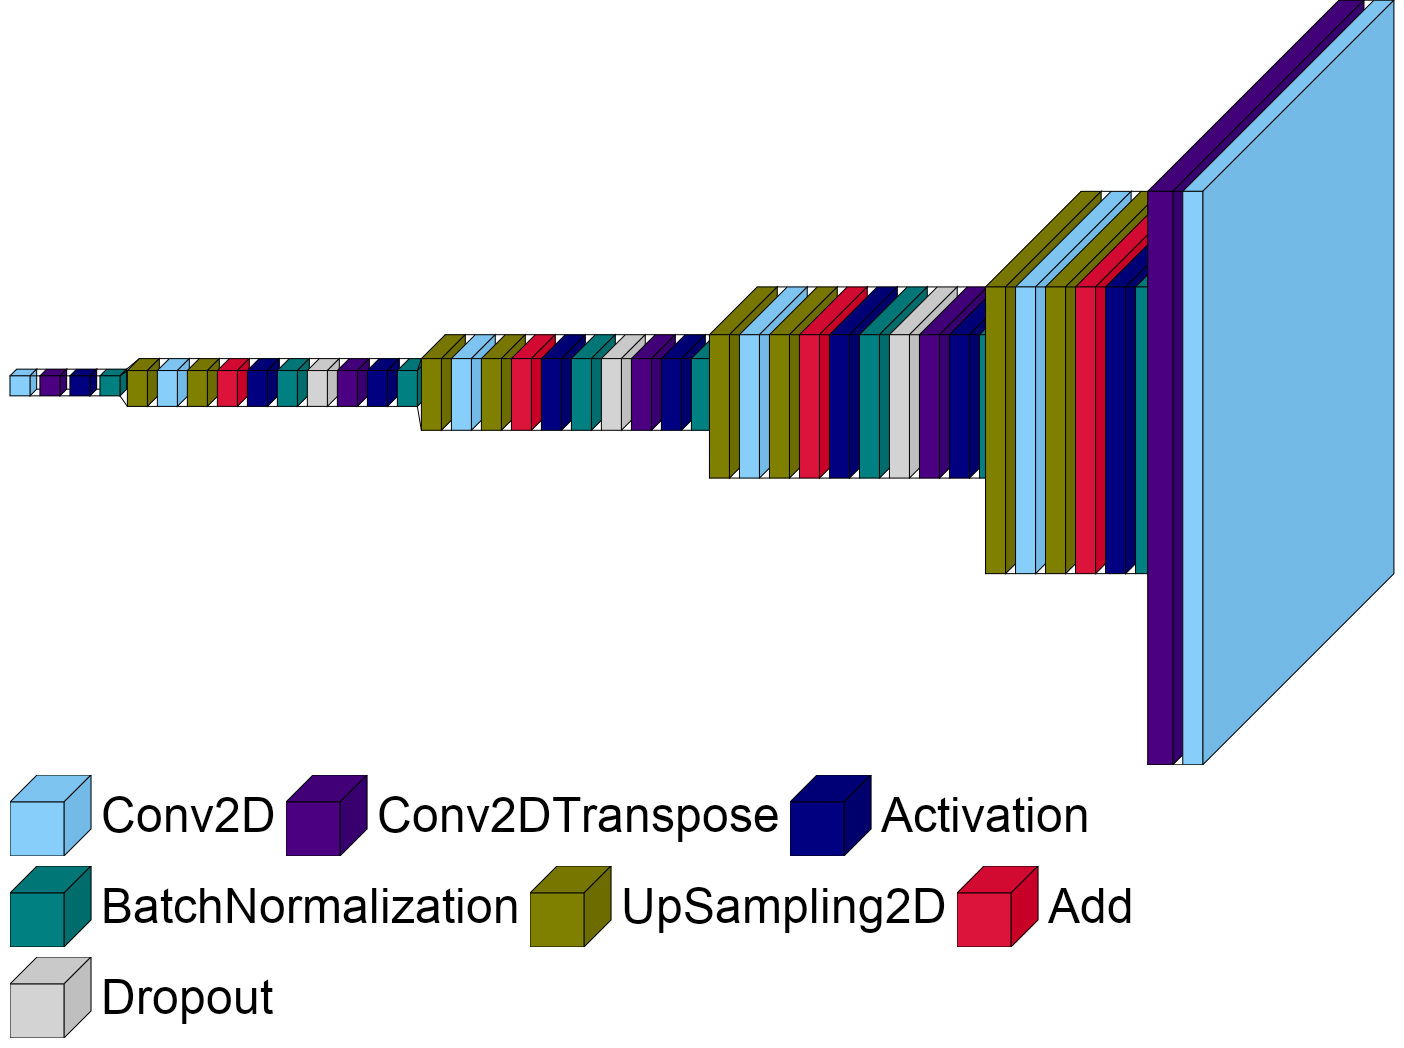
\includegraphics[width=0.7\textwidth]{Images/model_plot/advanced_decoder.png}
	\captionof{figure}{Architecture of the Advanced Decoder}
	\label{fig:Model_advanced_decoder}
\end{minipage}

\section{Final Segmentation Architecture with a Pre-trained Encoder}
For the final segmentation net, the U-Net architecture was combined with a \verb|MobileNetV2| pre-trained encoder. Also not all layers of the \verb|MobileNetV2| were used in order to keep the network small and slim. The skipped connections from the encoder were exported and added in the different decoder layers as it can be seen in \cref{lst:FinalNet}. This combination was trained in 50 epochs for a single-classification and a multi-classification.\\

\begin{minipage}[t]{\textwidth}
\centering
	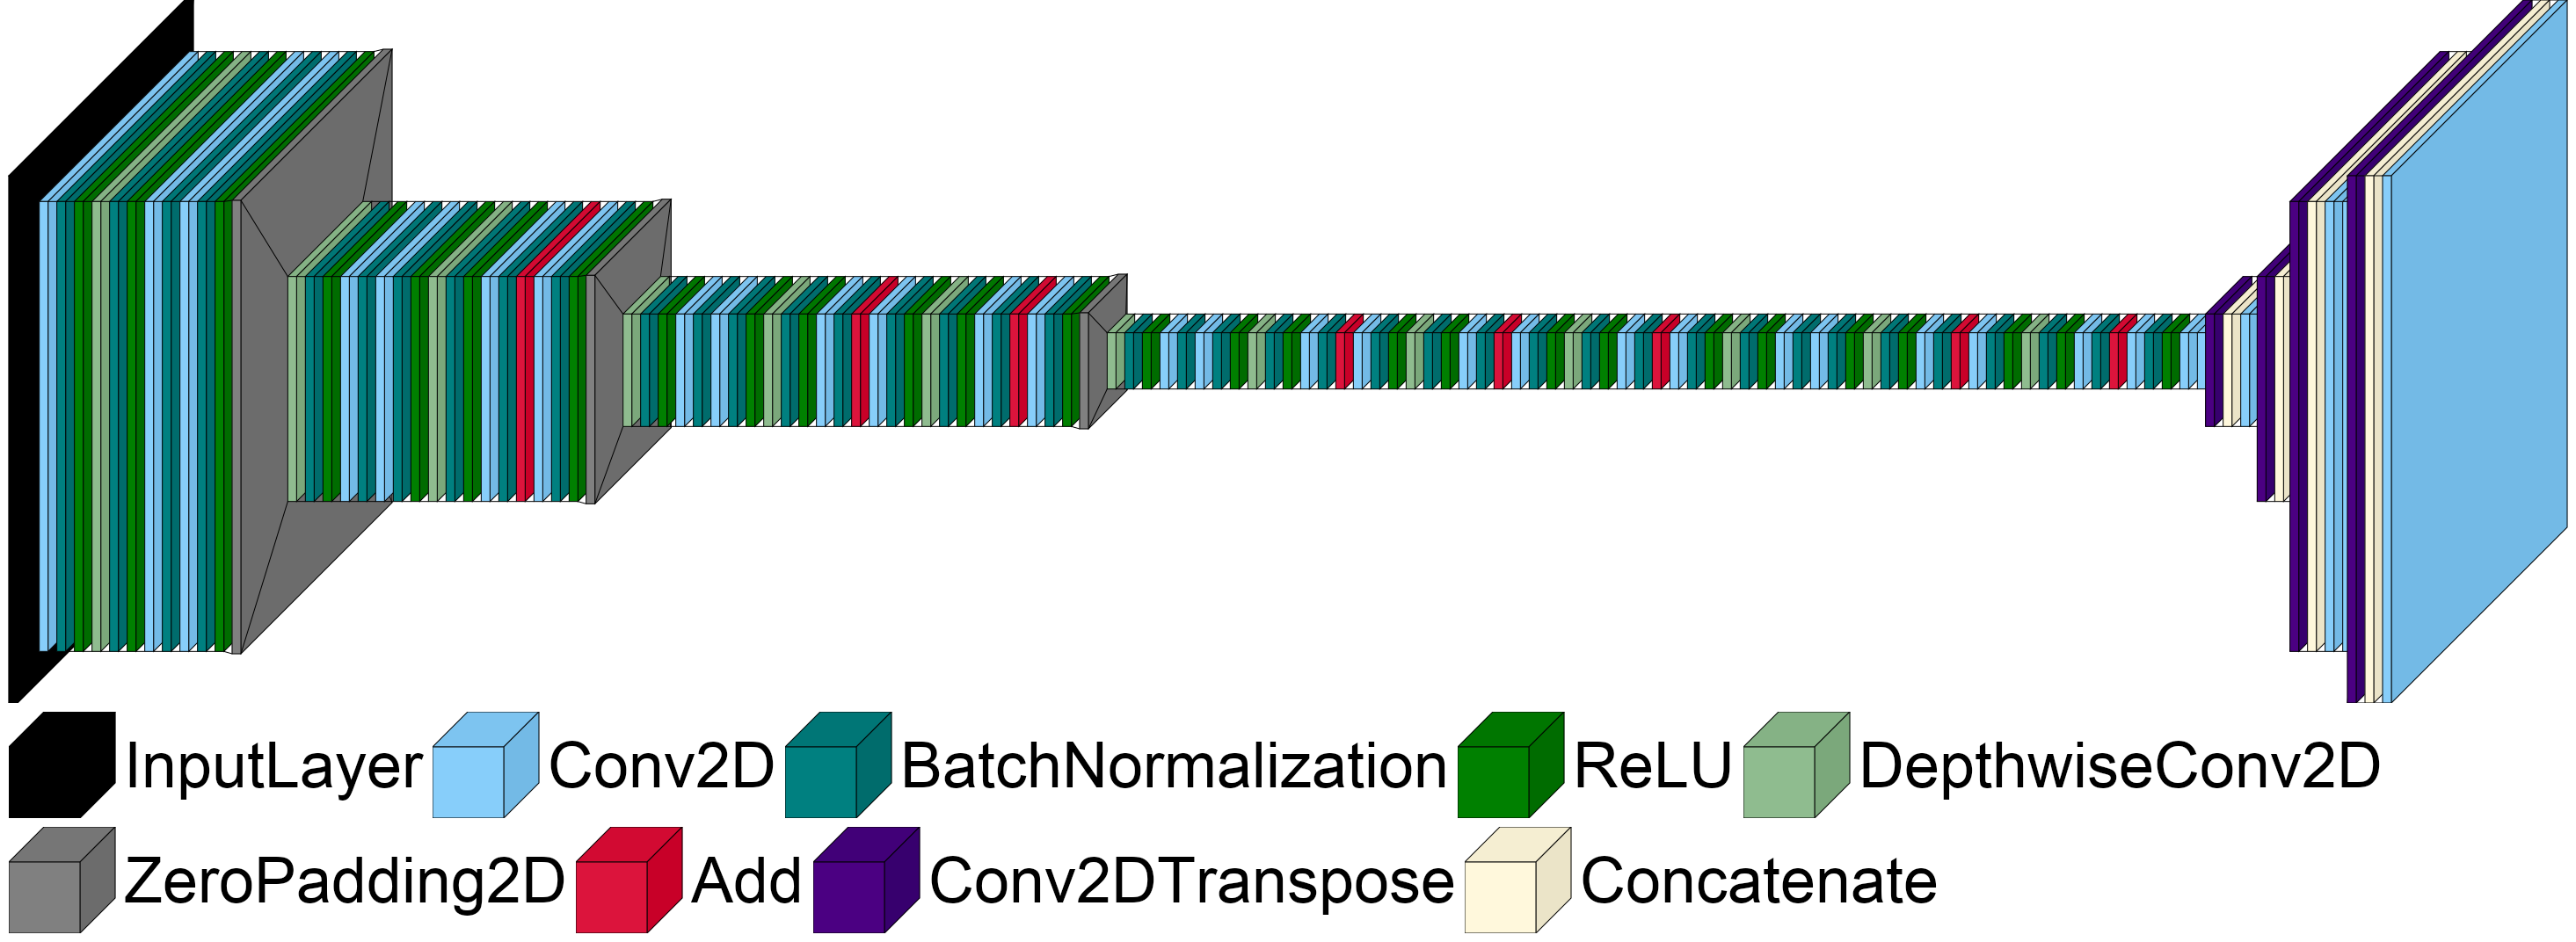
\includegraphics[width=\textwidth]{Images/model_plot/unet_mobilenet_v2.png}
	\captionof{figure}{Architecture of Final Model}
	\label{fig:Final_model}
\end{minipage}
